\clearpage
\subsection{RoPeR}
This chapter contains published interpretations of RoPeR data, with the latest update being May 2025. The purpose of this section is to look into GPR data from Mars, gathered by an instrument other than RIMFAX. 

\begin{table}[h!]
\centering
\caption{Grouped radar interpretation keywords extracted from the RoPeR dataset.}
\begin{tabular}{|p{6.8cm}|p{6.8cm}|}
\hline
\textbf{Geometry / Structure} & \textbf{Geometry / Structure (cont.)} \\
\hline
Dipping reflectors & Foreshore progradation \\
Domes & Matrix/clast layers \\
Hyperbolic reflections (point scattering) & Multidirectional dipping \\
Unidirectional dip & Parallel \\
Smooth interfaces & \\
\hline
\textbf{Amplitude / Reflectivity} & \textbf{Continuity} \\
\hline
High amplitude & Continuous reflectivity\\
Low frequency & Discontinuous reflections \\
Low reflectivity & Semi-continuous \\
Varied reflectivity\\
Strong reflectivity\\
\hline
\textbf{Terminations / Surfaces} & \textbf{Other / Descriptive} \\
\hline
Fining-upwards & Chaotic reflectors \\
Multilayered & \\
\hline
\end{tabular}
\label{tab:roper-keywords}
\end{table}

\subsubsection{Flood deposits}
\begin{figure}[h!]
    \centering
    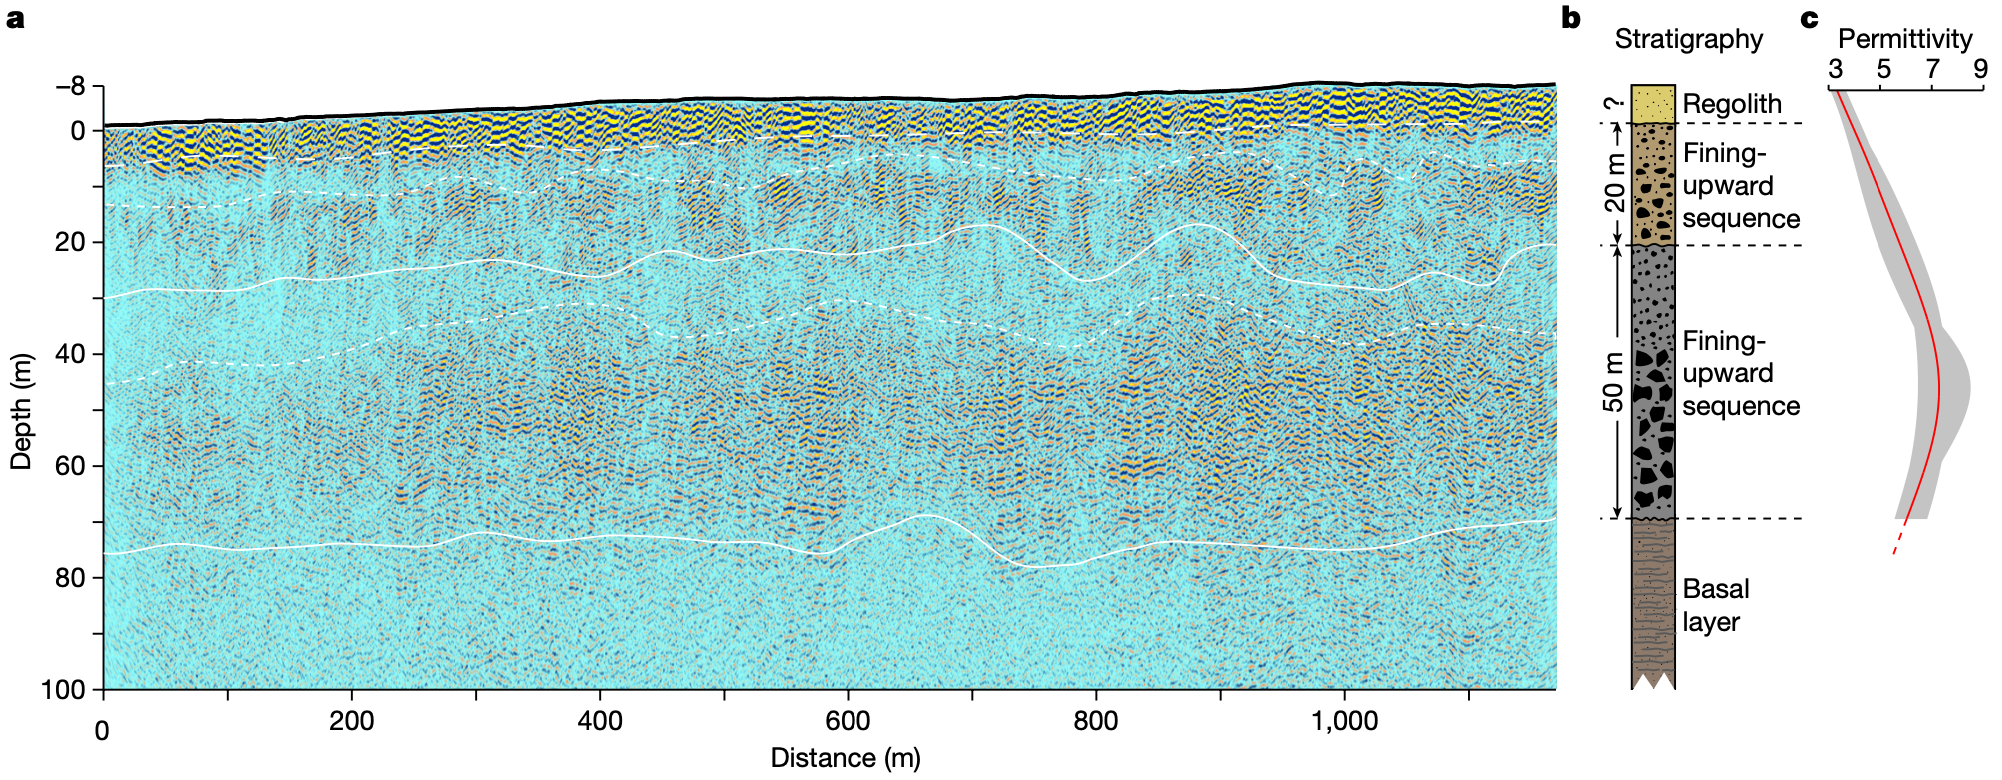
\includegraphics[width=0.9\linewidth]{Figures/0.6RoPeR/Li2022_1.png}
    \caption[Episodic hydraulic flooding sedimentation]{Episodic hydraulic flooding sedimentation \citep{Li2022}. \textbf{Keywords:} low-frequency, multi-layered, fining-upwards, Matrix/clast layers, discontinuous reflections, smooth interfaces. Weak to strong radar reflections with depth. Chaotic reflectors, multi-directional dipping.}
    \label{fig:Li2022-1}
\end{figure}
\clearpage
\subsubsection{Beach Ridge}
\begin{figure}[h!]
    \centering
    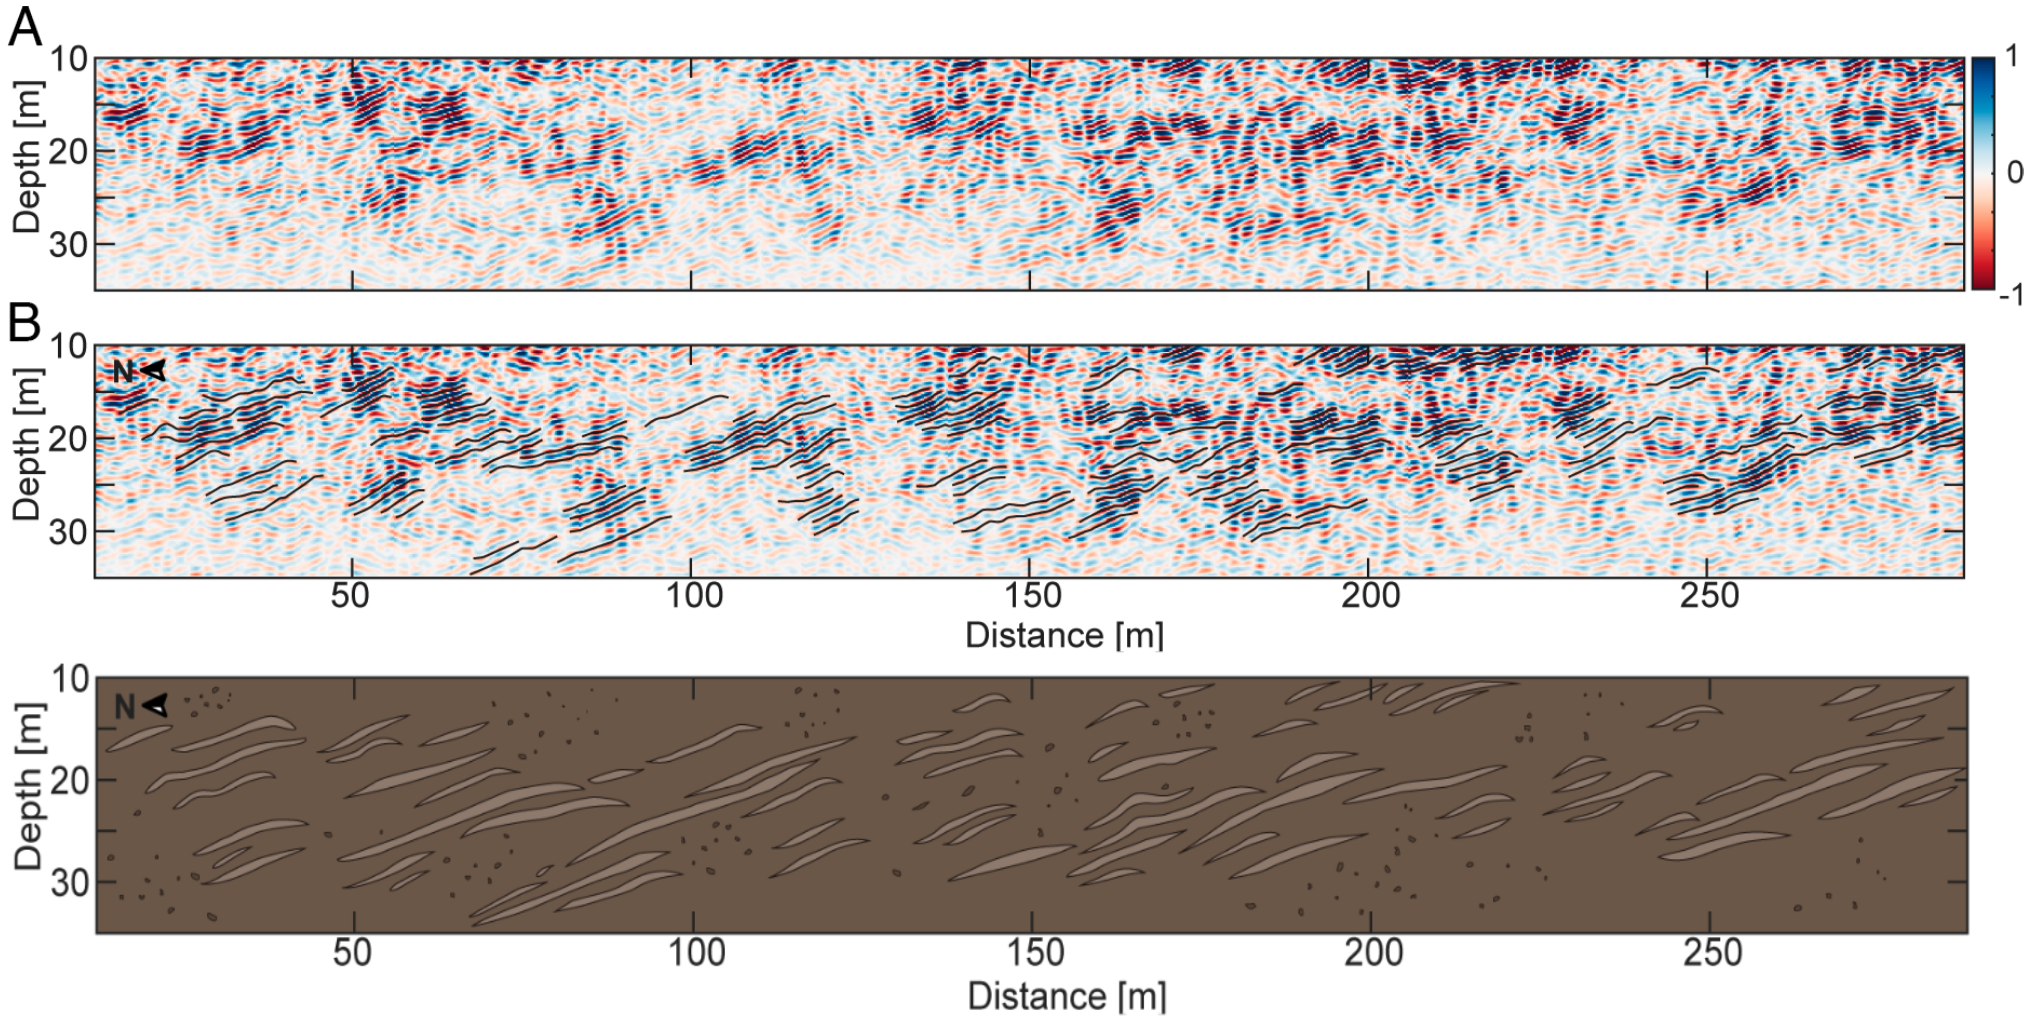
\includegraphics[width=0.9\linewidth]{Figures/0.6RoPeR/Li2025_1_3.png}
    \caption[Beach ridge deposits]{Beach ridge deposits, modified from \citep{Li2025}. \textbf{Keywords:} Dipping reflectors, unidirectional dip, multilayered, parallel, continuous reflectors, foreshore progradation, domes, hyperbolic reflections (point scattering).}
    \label{fig:Li2025-1-3}
\end{figure}

\begin{figure}[h!]
    \centering
    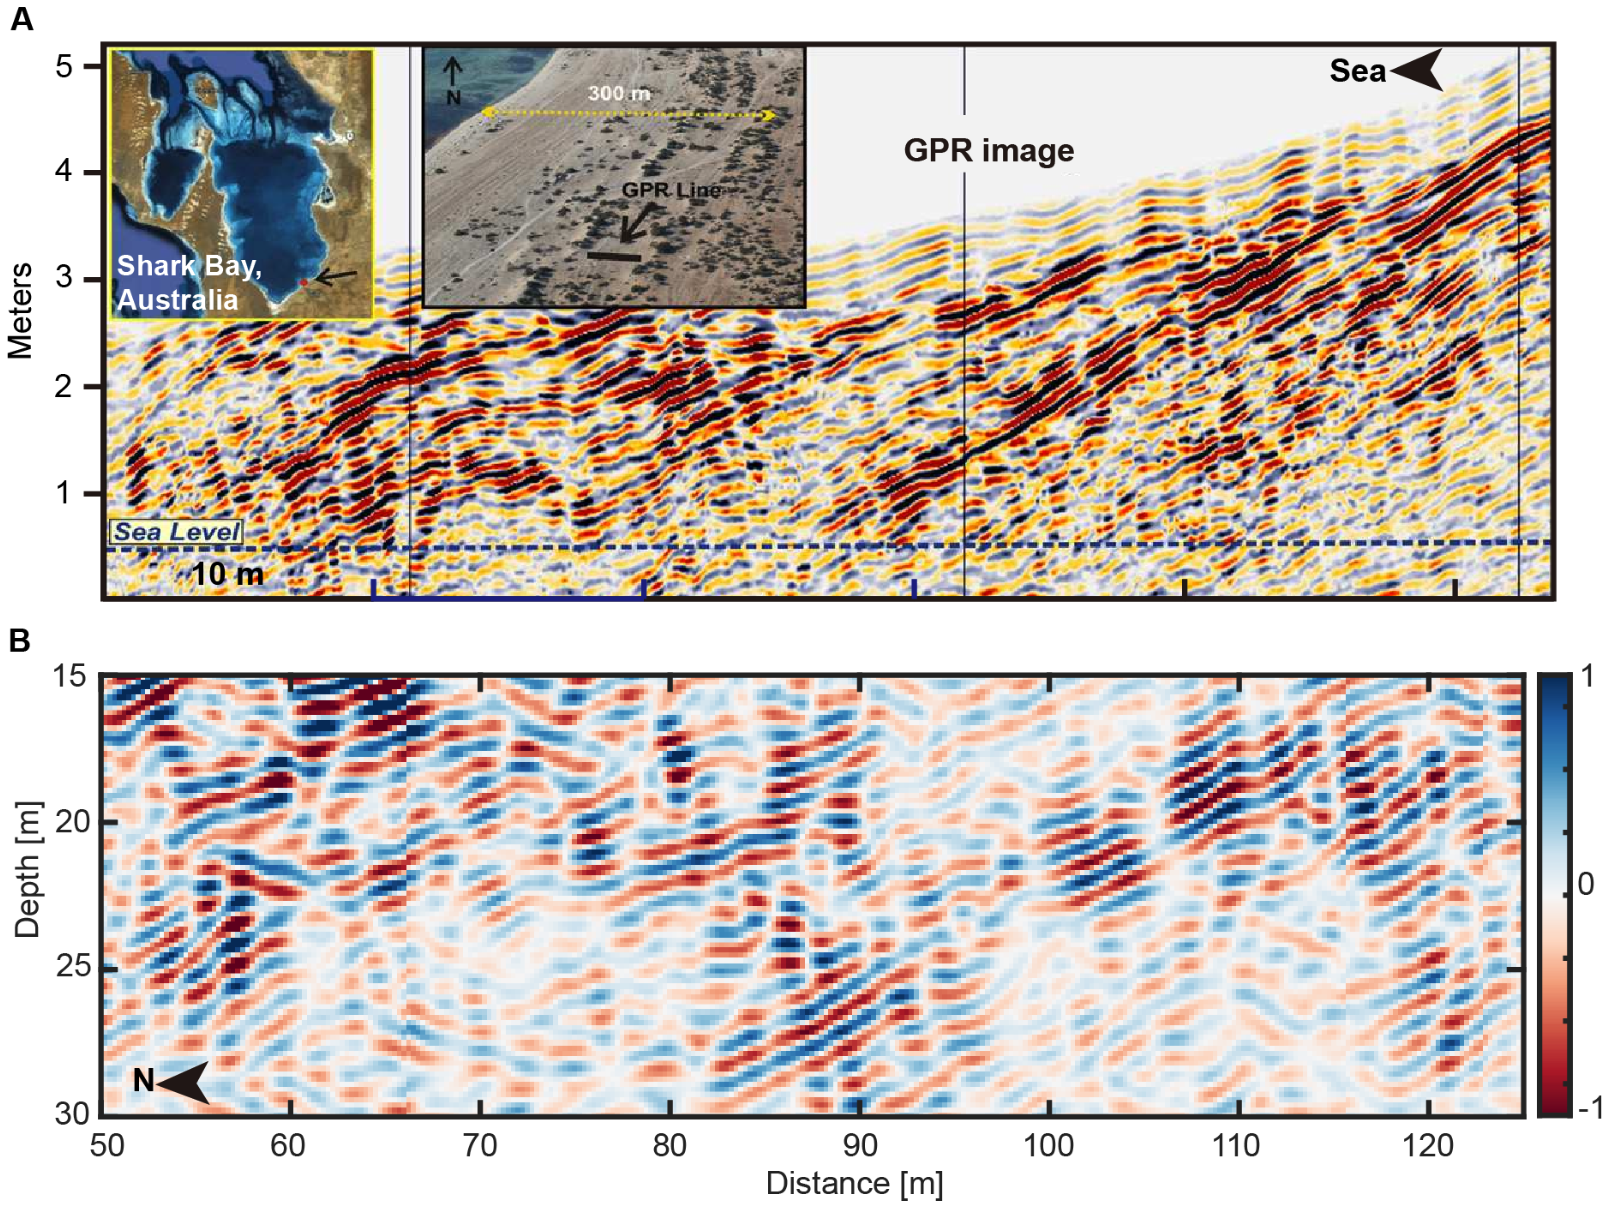
\includegraphics[width=0.9\linewidth]{Figures/0.6RoPeR/Li2025_2.png}
    \caption[Comparisons with Earth analogues to beach ridges]{Comparisons with Earth analogues to beach ridges \citep{Li2025}. \textbf{Keywords:} Unidirectional dipping, parallel, continuous, semi-continuous, sections of low-reflectivity, sections of strong reflectivity, multidirectional dipping.}
    \label{fig:Li2025-2}
\end{figure}